%%%% acra.tex

\typeout{ACRA Instructions for Authors}

% This is the instructions for authors for ACRA.
\documentclass{article}
\usepackage{acra}
\usepackage{lmodern}% http://ctan.org/pkg/lm
\usepackage{amsmath}
\usepackage{graphicx}
\usepackage{color}
\usepackage{hyperref}
\usepackage{amssymb}
\usepackage{url}
\usepackage{pdfpages}
\usepackage{fancyhdr}
\usepackage{subfig}
\usepackage{listings} 
\usepackage{selinput}    
\usepackage{tikz}
\usepackage[ruled,vlined]{algorithm2e}
\newcommand{\quotes}[1]{``#1''}

% The file acra.sty is the style file for ACRA. 
% The file named.sty contains macros for named citations as produced 
% by named.bst.

% The preparation of these files was supported by Schlumberger Palo Alto
% Research, AT\&T Bell Laboratories, and Morgan Kaufmann Publishers.
% Shirley Jowell, of Morgan Kaufmann Publishers, and Peter F.
% Patel-Schneider, of AT\&T Bell Laboratories collaborated on their
% preparation. 

% These instructions can be modified and used in other conferences as long
% as credit to the authors and supporting agencies is retained, this notice
% is not changed, and further modification or reuse is not restricted.
% Neither Shirley Jowell nor Peter F. Patel-Schneider can be listed as
% contacts for providing assistance without their prior permission.

% To use for other conferences, change references to files and the
% conference appropriate and use other authors, contacts, publishers, and
% organizations.
% Also change the deadline and address for returning papers and the length and
% page charge instructions.
% Put where the files are available in the appropriate places.

\title{Coordinate Ascent Variational Inference}
\author{Diego Garrido}

\begin{document}

\maketitle


Variational Inference (VI) is an approach used to approximate complicated distribution $p(z|x)$. It learn an approximate distribution $q(z)$ by optimization. In this paper, we use Coordinate Ascent Variational Inference (CAVI) to approximate the posterior distribution of a mixture of two 1D Gaussian distribution.

\href{https://nbviewer.jupyter.org/github/dgarridoa/CAVI/blob/main/CAVI.ipynb}{\color{blue}{Jupyter Notebook}}

\section{Gaussian Mixture Model}

Consider a 1D Gaussian mixture model with prior variance of component means $\sigma^{2}$. The full hierarchical model is

\begin{align}
    \mu_{k} &\sim \mathcal{N}(0, \sigma^{2}), & k=1,\ldots, K\\
    c_{i} &\sim Cat(1/K, \ldots, 1/K), & i=1, \ldots, n\\
    x_{i}|c_{i}, \mu &\sim \mathcal{N}(c_{i}^{T}\mu, 1) & i=1, \ldots, n
\end{align}


, and the mean-field variational family instead

\begin{align}
q(\mu, c) = \prod_{k=1}^{K}q(\mu_{k};m_{k}, s_{k}^{2})\prod_{i=1}^{n}q(c_{i};\varphi_{i})
\end{align}

\section{ELBO}

The Evidence Lower Bound (ELBO) to maximize is

\begin{align}
    &ELBO(m, s^{2}, \varphi) = \sum_{k=1}^{K}\mathbb{E}\big[\log p(\mu_{k});m_{k}, s_{k}^{2}\big]\\
    &+\sum_{i=1}^{n}\bigg(\mathbb{E}\big[\log p(c_{i});\varphi_{i}\big]+\mathbb{E}\big[\log p(x_{i}|c_{i}, \mu);\varphi_{i},m, s^{2}\big]\bigg)\\
    &-\sum_{i=1}^{n}\mathbb{E}\big[\log q(c_{i};\varphi_{i})]-\sum_{k=1}^{K}\mathbb{E}\big[\log q(\mu_{k};m_{k}, s_{k}^{2})]
\end{align}

Using that $q(\mu_{k}; m_{k}, s_{k}^{2}) = \mathcal{N}(\mu_{k};m_{k}, s_{k}^{2})$ and $q(c_{i};\varphi_{i})=Cat(c_{i};\varphi_{i})$ the ELBO can be written as

\begin{align}
    &ELBO(m, s^{2}, \varphi) = -\frac{1}{2\sigma^{2}}\sum_{k=1}^{K} m_{k}^{2}+s_{k}^{2}-\frac{1}{2}\log 2\pi\sigma^{2}\\
    &-n\log K+\sum_{i=1}^{N}\sum_{k=1}^{K}\varphi_{ik}(m_{k}x_{i}-\frac{m_{k}^{2}+s_{k}^{2}}{2})\\
    &-\frac{1}{2}\sum_{i=1}^{n}x_{i}^{2}-\frac{n}{2}\log 2\pi \\
    &-\sum_{i=1}^{n}\sum_{k=1}^{K}\varphi_{ik}\log \varphi_{ik}-\frac{1}{2}\sum_{k=1}^{K}\log s_{k}^{2}
\end{align}

, and can be simplified to 

\begin{align}
    &ELBO(m, s^{2}, \varphi) = -\frac{1}{2\sigma^{2}}\sum_{k=1}^{K} m_{k}^{2}+s_{k}^{2}\\
    &+\sum_{i=1}^{N}\sum_{k=1}^{K}\varphi_{ik}(m_{k}x_{i}-\frac{m_{k}^{2}+s_{k}^{2}}{2})\\
    &-\sum_{i=1}^{n}\sum_{k=1}^{K}\varphi_{ik}\log \varphi_{ik}-\frac{1}{2}\sum_{k=1}^{K}\log s_{k}^{2}\\
    &+const
\end{align}

, so we can omit the constant.

\section{CAVI}

Below the particular CAVI algorithm:

\begin{algorithm}[H]
    \SetAlgoLined
    \SetKwInOut{Input}{input}
    \SetKwInOut{Output}{output}
    \SetKwInOut{Init}{initialize}
    \Input{Data $x_{1:n}$, number of components $K$, prior variance of component means $\sigma^{2}$}
    \Output{Variational densities $q(\mu_{k};m_{k},s_{k}^{2})$(Gaussian) and $q(c_{i};\varphi_{i})$ (K-categorical)}
    \Init{Variational parameters $m=m_{1:K}$, $s^{2}=s_{1:K}^{2}$, and $\varphi=\varphi_{1:n}$}
    \While{the ELBO has not converged}{
        \For{$i \in\{1,\ldots, n\}$}{
            Set $\alpha_{ik} = \exp\big(m_{k}x_{i}-\frac{m_{k}^{2}+s_{k}^{2}}{2}\big)$\\
            Set $\phi_{ik} = \frac{\alpha_{ik}}{\sum_{k=1}^{K}\alpha_{ik}}$
        }
        \For{$k \in \{1, \ldots, K\}$}{
            Set  $m_{k} = \frac{\sum_{i=1}^{n}\varphi_{ik}x_{i}}{1/\sigma^{2}+\sum_{i=1}^{n}\varphi_{ik}x_{i}}$\\
            Set $s_{k}^{2} = \frac{1}{1/\sigma^{2}+\sum_{i=1}^{n}\varphi_{ik}x_{i}}$
        }
     }
     \caption{CAVI}
     Compute ELBO($m, s^{2}, \varphi$)
\end{algorithm}

The convergence criterion used is $ELBO_{i}-ELBO_{i-1}<tol$ and $ELBO_{i}-ELBO_{i-1}\geq 0$, where $tol$ means the numerical tolerance, in this case it was set to $1e-16$. 

\section{Data}

In this section is explained the process used to generate the data. Firstly, was setted the number of components to discover in $K=2$ and the prior variance of component means in $\sigma^{2}=100$. Secondly, two means are sampled using $\mu_{k}\sim \mathcal{N}(0, \sigma)$. The means gotten are $\mu_{1}=2.210$ and $\mu_{2}=-3.405$. Thirdly, the mixtures components are sampled using $\pi\sim Dir(1_{K})$ and the clusters assignments from $c_{i}\sim Cat(\pi)$ with $i \in {1\,\ldots, n}$, where the sample size $n$ is not fixed. The $\pi$ gotten is $[0.656, 0.344]$. Finally, the data is sampled using $x_{i}|c_{i}, \mu \sim \mathcal{N}(c_{i}^{T}\mu, 1)$. It is ilustrated in Figure 1 using a sample size $n=10000$. 

\begin{figure}[!h]
    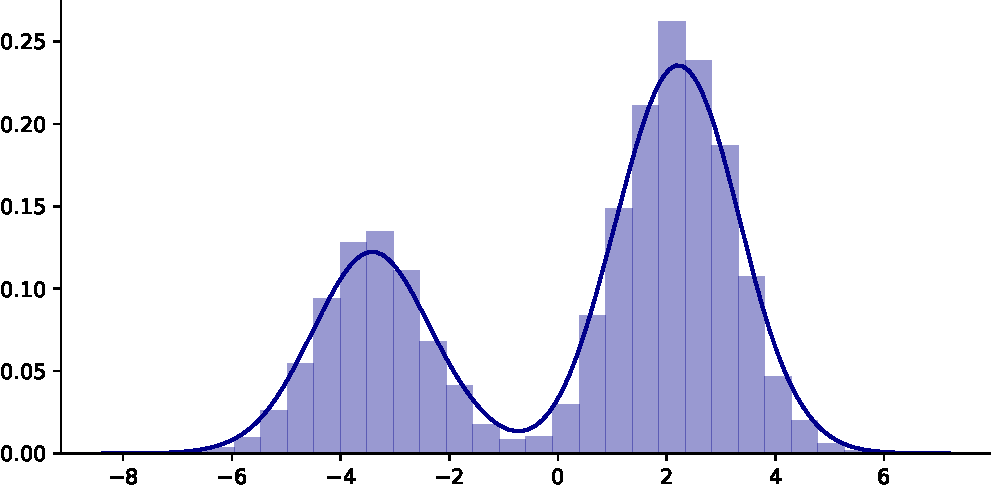
\includegraphics[width=0.5\textwidth]{img/data.pdf} 
    \caption{Random sample of a mixture of two Gaussians with sample size $n=10000$.}
\end{figure}

\section{ELBO convergence}

This section shows ELBO's convergece in function of different samples sizes and initial parameters. The ELBO's convergence for different sample sizes is illustrated in Figure 2. The initial variational parameters used are the same, they are $m_{k} = 0$ (the prior mean), $s_{k}=1$ and $\phi_{ik}=1/K$. In this figure it is observed that the greater sample size takes less iterations in converge. However, a larger sample size implies more expensive iterations. The behavior of the ELBO's convergence for different initial variational parameter is shown in Figure 3. The sample size used are the same and is $n=100$. In this figure it is observed that different initialization of the variational parameters may lead CAVI to find different local optima of the ELBO.


\begin{figure}[!h]
    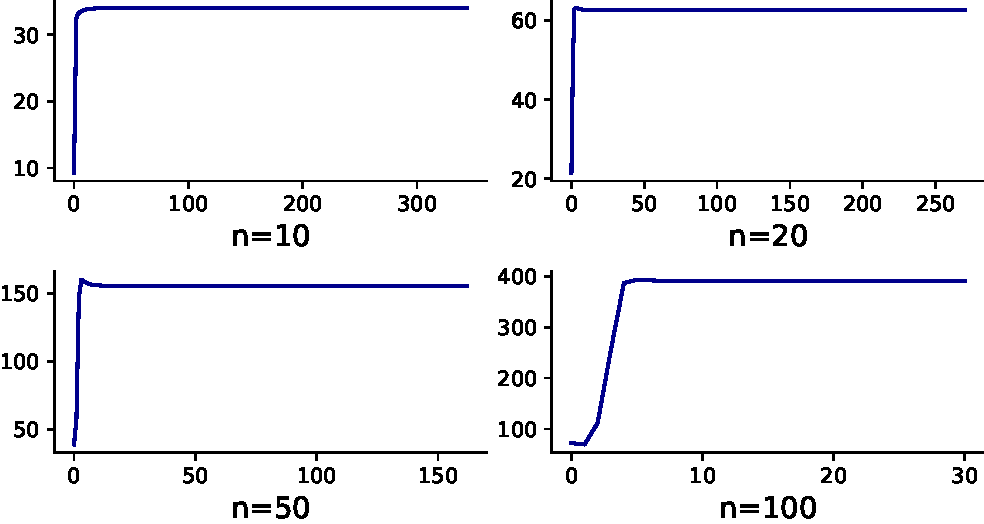
\includegraphics[width=0.5\textwidth]{img/elbo_sample.pdf} 
    \caption{Iteration that the ELBO takes to converge for different sample sizes.}
\end{figure}

\begin{figure}[!h]
    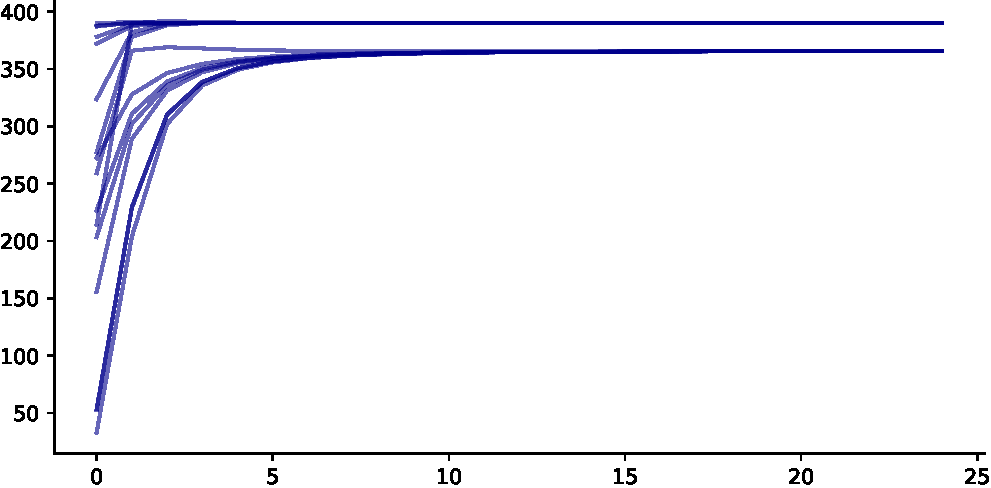
\includegraphics[width=0.5\textwidth]{img/elbo_init.pdf} 
    \caption{The ELBO using different initial variational parameters on CAVI.}
\end{figure}

\section{CAVI approximation}

The mean-field approximation is shown in Figure 4. In this figure can be senn that the mean-field approximation underestimate the posterionr variance. This is consequence of its objective function, since it penalizes more to put mass in regions where $p(z|x)$ has no mass. Despite underestimating the variance, the approximation is quite good, where for a sample size $n=100$ the expected value of the means are $\mathbb{E}(\mu_{1}) = 2.064$ and $\mathbb{E}(\mu_{2})=-3.689$, very close to the means used to generate the data.

\begin{figure}[!h]
    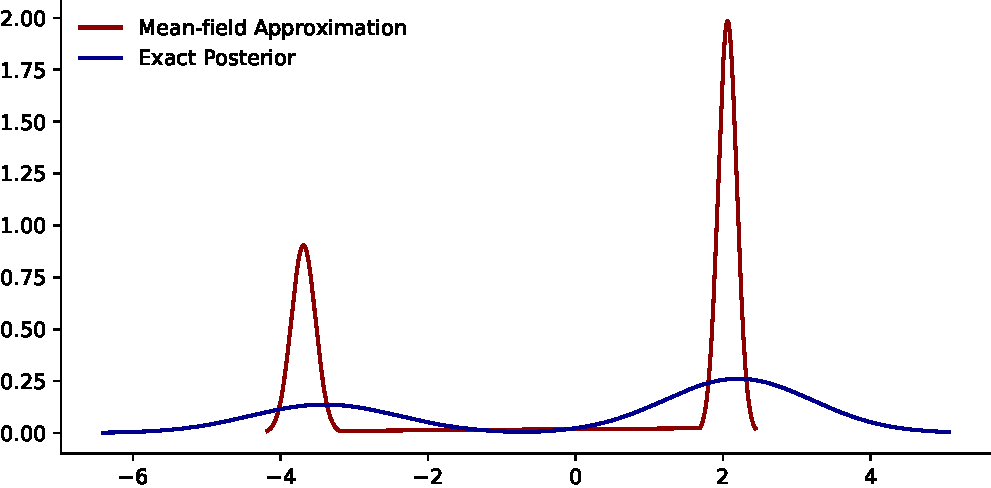
\includegraphics[width=0.5\textwidth]{img/cavi_approx.pdf} 
    \caption{Mean-field approximation of a Gaussian mixture model.}
\end{figure}

\end{document}